\documentclass{article}
\usepackage{graphicx} % Required for inserting images
\usepackage{minted}

\title{Exploring Results in Differential Geometry}
\author{Alex Zhou}
\date{May 2019}

\begin{document}

\maketitle

\section{Introduction}

A curve in the complex plane is a continuous map \(\gamma\) from the closed bounded interval \([a,b] \subset \mathbf{R}\) to \(\mathbf{C}\). We say that \(\gamma\) is smooth if \(\gamma(t) = (u(t), v(t))\) for smooth functions \(u, v\) and \(\gamma\) is closed if \(\gamma(a) = \gamma(b)\).

Suppose that \(w = f(z)\) is a complex polynomial in \(z\) and  \(r > 0\). If \(C_r\) is the circle of radius \(r\) then it must be the case that the image \(f(C_r)\) is a smooth closed curve in the \(w\)-plane. Curves that are generated in this way have a number of interesting properties that will try to derive.

\section{Root of Polynomials}

Let \(f_1(z) = z^3 - z^2 + (2 - i)z - 1 - i\). The following program generates the values of the curve \(f(C_r)\) and also computes an approximation for the closest point on the curve to to origin.

\begin{minted}[autogobble, linenos]{python}
    def find_curve_values(f, r, resolution = 10000):
        theta_values = np.linspace(0, 2 * np.pi, resolution)
        circle_values = r * np.exp(1j * theta_values)
        return circle_values, f(circle_values)
    
    def find_min_modulus_point(circle_values, curve_values):
        min_index = np.argmin(np.abs(curve_values))
        return circle_values[min_index], curve_values[min_index]
\end{minted}

The curve and point with smallest absolute value can then be plotted.

\begin{figure}
    \centering
    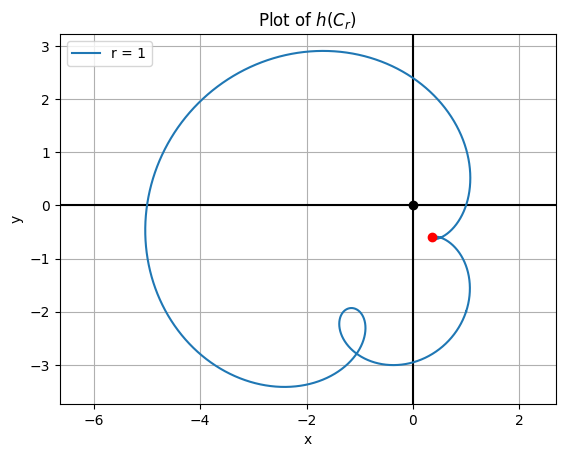
\includegraphics[width=0.75\linewidth]{images/curvef1.png}
    \caption{Plot of the curve \(f(C_1)\).}
\end{figure}

Recall Rouche's theorem which states that for a given polynomial \( \sum_{i=0}^n a_nz^n\), if there exists \(R > 0\) and \(k \in \mathbf{N}\) such that
\[ |a_k|R^k > |a_0| + \dots + |a_{k-1}|R^{k-1} + |a_{k+1}|R^{k+1} + \dots |a_n|R^n, \]
then there are exactly \(k\) roots (counted with multiplicity) inside \(C_R\). In our case, taking \(k = 3\) and \(R = 3\), we have the inequality
\[ 27 = |a_3|R^3 > 18 > |a_0| + |a_1|R + |a_2|R^2 = \sqrt{2} + \sqrt{5}\cdot3 + 1\cdot3^2, \]
which implies that all three roots of \(f_1\) lie inside \(C_3\). By considering the reciprocal polynomial \(\sum_{i=0}^n a_{n-i}z^n\), the roots of this polynomial are reciprocals of the roots of the original polynomial, hence an upper bound for the roots of the reciprocal polynomial yields a lower bound for the roots of the original polynomial. A similar calculation shows that the roots of \(f_1\) lie outside the circle \(C_{1/3}\). Running our algorithm with \(r\) in this range with step-size \(10^{-4}\) and sufficiently high resolution, we find three roots at
\[ z_1 \approx 0.618i, \quad z_2 \approx 1+i, \quad z_3 \approx -1.618i, \]
which is correct up to a tolerance and error of \(10^{-3}\). The former is justified by testing nearby values and the latter by direct substitution.

The derivative of \(f_1\) is clearly
\[ f_1'(z) = 3z^2 - 2z + 2 - i. \]
We can directly use Rouche's theorem again to prove that the two roots lie within the circles \(C_{1/2}\) an \(C_2\). Applying the same procedure as before, we obtain the roots
\[ z_4 = 0.118 - 0.776i, \quad z_5 = 0.548 + 0.776i, \]
correct up to tolerance and error \(10^{-3}\) using the same verifications.

\section{The Geometry of the Image of a Circle}

Consider the polynomial
\[ g(z) = z^3 + z. \]
When \(|z| = r\) is very small, the \(z^3\) term is dominated by the \(z\) term, so asymptotically, \(g(z) \approx z\). Thus, for small \(r\), the image \(g(C_r)\) is a simple, nearly circular curve centred at the origin whose shape and radius closely resembles the shape of the original circle \(C_r\). The behaviour of the mapping may change significantly at critical points where the derivative is zero. Also, when \(r\) matches the modulus of a root of \(g\), we expect the curve to intersect with the origin. Since 
\[ g'(z) = 3z^2 + 1, \]
we have critical points at \(z = \pm i/\sqrt3\). Hence, the critical modulus or radius is \(r = 1/\sqrt{3}\).
\begin{enumerate}
    \item Small \(r\) leads to a curve closely resembling a circle, as illustrated above.
    \item As \(r\) approaches \(1/\sqrt{3} \approx 0.577\), the curve becomes less circular, and shows two indentations.
    \item For \(r = 1/\sqrt{3}\), the circle \(C_r\) passes directly through the critical points. At the images of the critical points, the curve \(g(C_r)\) forms cusps where the curve fails to be differentiable.
    \item When \(r\) exceeds \(1/\sqrt{3}\), the circle \(C_r\) now encloses the critical points and the image \(g(C_r)\) is no longer simple since it develops self-intersections.
    \item Finally, when \(r\) is large, in particular \(r > 1\), the \(z^3\) term dominates and the curve winds around the origin three times. We see that the edge case \(r = 1\), the inner loops touch the origin due to the double roots \(\pm i\).
\end{enumerate}

\begin{figure}
    \centering
    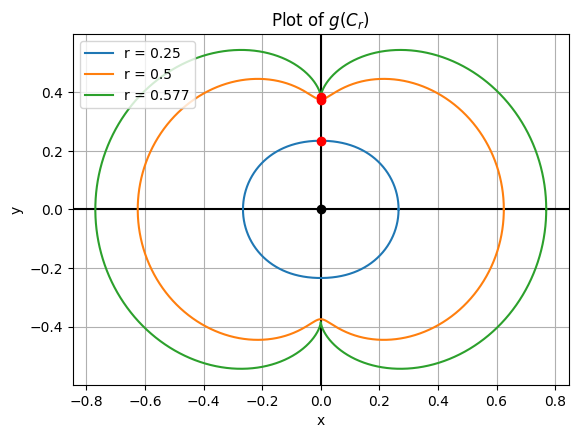
\includegraphics[width=0.49\linewidth]{images/smallr.png}
    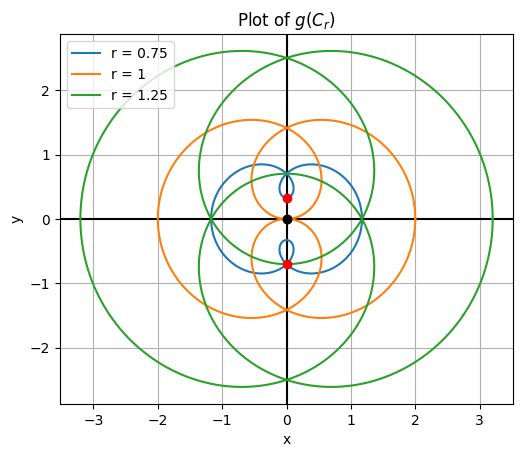
\includegraphics[width=0.49\linewidth]{images/larger.png}
    \caption{Plot of \(g(C_r)\) for small and large \(r\).}
\end{figure}

Now consider
\[ h(z) = z^3 - z^2 - z + 1. \]
A similar analysis of the critical points now yield two moduli, namely the radii \(r = 1/3\) and \(r = 1\).
\begin{enumerate}
    \item For small \(r\), \(1 - z\) dominates and \(C_r\) approximates a circle around the origin.
    \item As \(r\) approaches \(1/3\), \(h(C_r)\) distorts and develops an indentation.
    \item At \(r = 1/3\), the circle \(C_r\) passes through the critical point \(-1/3\) and the curve \(h(C_r)\) develops a cusp at \(h(-1/3) = 32/37 = 1.185\).
    \item As \(r\) approaches \(1\), the cusp opens up into a self-intersecting loop and the curve approaches the origin.
    \item At \(r = 1\), we now see a cusp at the origin as the circle \(C_r\) passes through the critical point \(1\) and \(h(1) = 0\) and the curve also has a triple root at the origin.
    \item When \(r\) grows beyond \(1\), the circle \(C_r\) encloses both critical points, the cusp at the origin opens up, forming a second loop and the \(z^3\) term dominates, leading to the curve winding around \(1\) three times.
\end{enumerate}

\begin{figure}
    \centering
    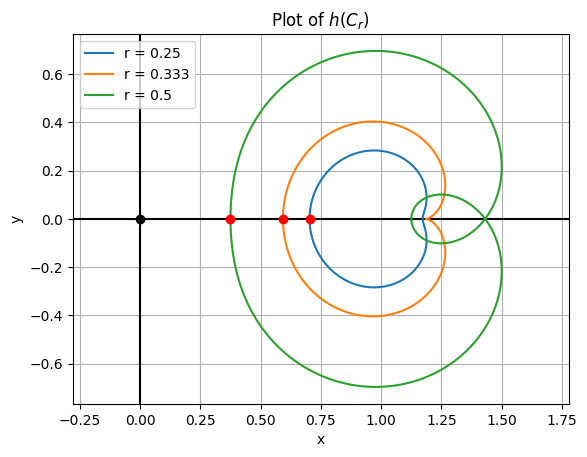
\includegraphics[width=0.49\linewidth]{images/hsmallr.png}
    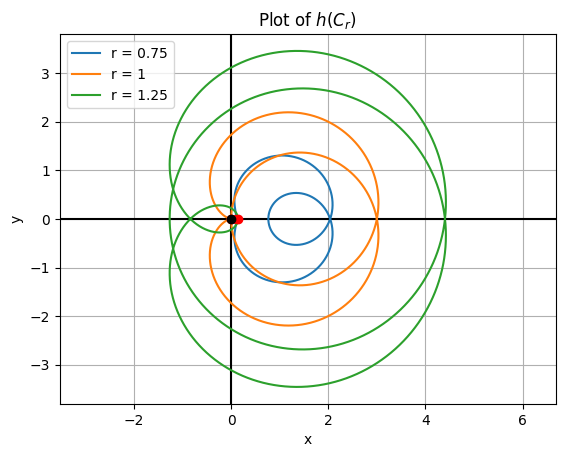
\includegraphics[width=0.49\linewidth]{images/hlarger.png}
    \caption{Plot of \(h(C_r)\) for small and large \(r\).}
\end{figure}

Looking back at 
\[ f_1(z) = f_1(z) = z^3 - z^2 + (2 - i)z - 1 - i, \]
we can show that the exact roots for \(f_1\) are at \(z = i(\phi-1), 1+i, -i\phi\), where \(\phi = \frac{\sqrt{5} + 1}{2}\) is the golden ratio. The approximate critical points are
\[ z_4 = 0.118 - 0.776i, \quad z_5 = 0.548 + 0.776i, \]
which have approximate modulus \(0.7847\) and \(0.949\) respectively. 

From the previous analysis of \(g\) and \(h\), the modulus of the roots of \(f_1\) correspond to curves that intersect the origin; the modulus of critical points of \(f_1\) correspond to cusps and the opening of loops; small values of \(r\) lead to simple approximations of a circle (\(z\) dominates) centred at the constant term \(-1 - i\); and large values of \(r\) result in the \(z^3\) term dominating, giving the curve a winding number of \(3\).

\begin{figure}
    \centering
    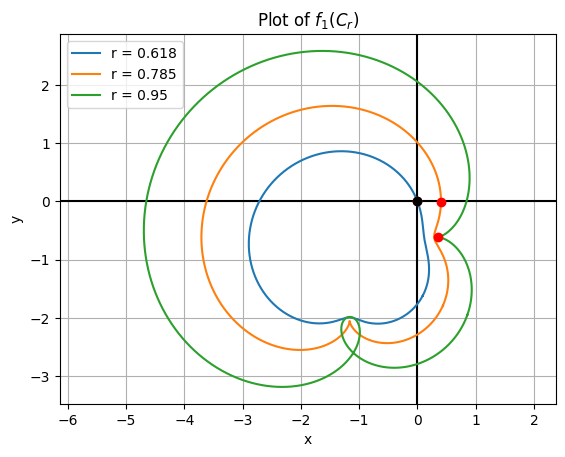
\includegraphics[width=0.49\linewidth]{images/fsmallr.png}
    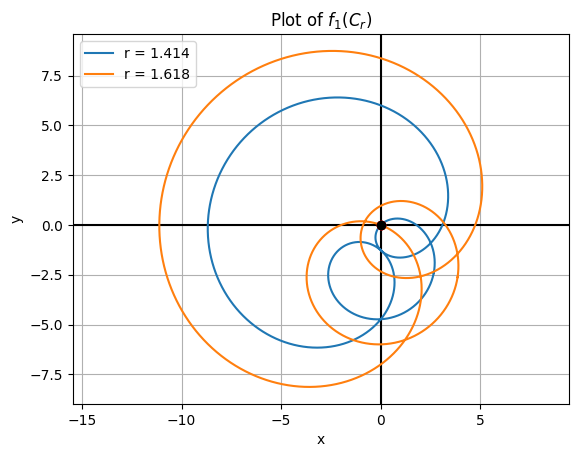
\includegraphics[width=0.49\linewidth]{images/flarger.png}
    \caption{Plot of \(f_1(C_r)\) for small and large \(r\).}
\end{figure}

\section{Curvature of Curves}

A smooth curve \(\mathbf{x}: [a,b] \to \mathbf{C}\) is said to be regular if \(\mathbf{x}'(t) \neq 0\) for all \(t \in [a, b]\). From the inverse function theorem (or implicit function theorem), any smooth regular curve admits a smooth reparametrisation (also denoted \(\mathbf{x}\) by abuse of notation) such that the parameter \(s\) is equal to the distance travelled along the curve. This is regarded as the natural parametrisation and is usually called the arc-length parametrisation. The distance from \(\mathbf{x}(s)\) to \(\mathbf{x}(s+ds)\) is
\[ dx = |\mathbf{x}(s+ds) - \mathbf{x}(s)|, \]
for some infinitesimal \(ds\) along the curve. Thus \(|\dot{\mathbf{x}}(s)| = 1\) for all \(s\), where
\[ \dot{\mathbf{x}}(s) = \lim_{ds \to 0} \frac{\mathbf{x}(s+ds) - \mathbf{x}(s)}{ds}. \]
The unit tangent vector at \(s\) is \(\mathbf{t}(s) = \dot{\mathbf{x}}(s)\). The curvature vector of the curve at \(s\) is defined as \(\mathbf{k}(s) = \ddot{\mathbf{x}}(s)\) and the curvature of the curve at \(s\) is 
\[ |\kappa| = |\mathbf{k}(s)|, \]
and the radius of curvature is \(\rho = 1/|\kappa|\). Typically, the function \(f(z)\) is not a natural representation of the curve \(f(C_r)\) as \(z\) is not a scalar and it is not the case that \(z_2-z_1\) is the distance in \(\mathbf{C}\) along the curve between \(f(z_1)\) and \(f(z_2)\). However, by using suitable coordinate transforms, an expression for the curvature vector can be found for an arbitrary parametric representation \(f(z)\).

Write \(f(z)\) in terms of the angle \(\varphi = \arg z\) to give a representation \(\mathbf{x} = \mathbf{x}(\varphi)\) of the curve \(f(C_r)\) in terms of \(\varphi\),
\begin{eqnarray*} 
    x(\varphi) = \Re[f(z(\varphi))]  = \Re[f(\varphi)] \\
    y(\varphi) = \Im[f(z(\varphi))]  = \Im[f(\varphi)]
\end{eqnarray*}
where \(\mathbf{x}(\varphi) = (x(\varphi), y(\varphi))\). Recall that the curvature of a parametric plane curve is given by
\[ |\kappa| = \frac{|x'y'' - y'x''|}{((x')^2 + (y')^2)^{3/2}} = \frac{|\mathbf{x}' \times \mathbf{x}''|}{|\mathbf{x}'|^3}, \]
where 
\[ \mathbf{x}'(\varphi) = \left( \Re\left[\frac{df(z(\varphi))}{d\varphi}\right], \ \Im\left[\frac{df(z(\varphi))}{d\varphi}\right] \right) \]
and
\[ \mathbf{x}''(\varphi) = \left( \Re\left[\frac{d^2f(z(\varphi))}{d\varphi^2}\right], \ \Im\left[\frac{d^2f(z(\varphi))}{d\varphi^2}\right] \right) \]
We define the sign of \(\kappa\) to be positive if \(\mathbf{x}(s)\) turns anti-clockwise with respect to its local centre of rotation. This can be determined from the sign of \(\mathbf{x}' \times \mathbf{x}''\) which determines the sign of the angle between the unit tangent (which is proportional to the derivative) and the unit normal vector (which is proportional to the curvature vector, hence the second derivative).

For \(z(\varphi) = re^{i\varphi}\), we have
\[ \frac{dz}{d\varphi} = ire^{i\varphi} = iz(\varphi), \]
which gives
\[ \frac{df(z(\varphi))}{d\varphi} = \frac{df}{dz}(z(\varphi))\frac{dz}{d\varphi} = if'(z(\varphi))z(\varphi), \]
so
\[ \mathbf{x}'(\varphi) = \left( \Re[if'(z(\varphi))z(\varphi)], \ \Im[if'(z(\varphi))z(\varphi)] \right). \]
Furthermore,
\[ \frac{d^2f(z(\varphi))}{d\varphi^2} = \frac{d[if'(z(\varphi))z(\varphi)]}{d\varphi} = -z(\varphi) f'(z(\varphi)) - z(\varphi)^2f''(z(\varphi)), \]
which yields,

\begin{eqnarray*}
    &&\mathbf{x}''(\varphi) =\\
    && \left( \Re[-z(\varphi) (f'(z(\varphi)) + f''(z(\varphi))z(\varphi))], \ \Im[-z(\varphi) (f'(z(\varphi)) + f''(z(\varphi))z(\varphi))] \right)
\end{eqnarray*}
as required. 


Now define the total curvature over the curve \(C_r\) as
\[ \kappa_{\mathrm{tot}} = \int_{f(C_r)} \kappa \,ds. \]
We have the signed curvature with respect to \(\varphi\) which is defined as
\[ \kappa(\varphi) = \frac{\mathbf{x}'(\varphi) \times \mathbf{x}''(\varphi)}{|\mathbf{x}'(\varphi)|^3}. \]
Also \(ds = |\mathbf{x}'(\varphi)|d\varphi\). Thus
\begin{eqnarray*}
    \kappa & = & \int_0^{2\pi} \kappa(\varphi) \frac{ds}{d\varphi}\,d\varphi \\
           & = & \int_0^{2\pi} \frac{\mathbf{x}'(\varphi) \times \mathbf{x}''(\varphi)}{|\mathbf{x}'(\varphi)|^3} |\mathbf{x}'(\varphi)|\,d\varphi \\
           & = & \int_0^{2\pi} \frac{\Im(\overline{\mathbf{x}'(\varphi)}\mathbf{x}''(\varphi))}{|\mathbf{x}'(\varphi)|^2} \,d\varphi. \\
\end{eqnarray*}
To approximate this integral, for a given polynomial \(f\), we need to first compute the derivatives \(f'\) and \(f''\) as a means to compute \(\mathbf{x}'(\varphi)\) and \(\mathbf{x}''(\varphi)\). This can be used to calculate the integrand which is numerically integrated with respect to \(\varphi\) over \([0, 2\pi]\). We use the following program which uses SciPy numerical integration to compute an approximation to the integral.

\begin{minted}[autogobble, linenos]{python}
    def curvature_integrand(f_prime, f_double_prime, r, phi):
        z = r * np.exp(i * phi)
        f_prime_z = f_prime(z)
        f_double_prime_z = f_double_prime(z)
    
        x_prime_z = i * z * f_prime_z
        x_double_prime_z = -z * (f_prime_z + z * f_double_prime_z)
        
        numerator = np.imag(np.conj(x_prime_z) * x_double_prime_z)
        denominator = np.abs(x_prime_z)**2
        if denominator == 0:
            return 0
        return numerator / denominator
    
    def compute_total_curvature(f_prime, f_double_prime, r):
        if r == 0:
            return 0
        integrand = lambda phi: 
            curvature_integrand(f_prime, f_double_prime, r, phi)
        total_curvature, error = 
            integrate.quad(integrand, 0, 2 * np.pi, limit = 100)
        return total_curvature    
\end{minted}

We note that in the following plot of the total curvature of \(f_1\), \(g\) and \(h\) that there are jump discontinuities at the modulus of each critical point, counted with multiplicity. In fact, dividing by \(2\pi\) yields the turning number of the curve, which increases by \(1\) each time we pass through a cusp. Therefore, the expected turning number of the curve is equal to the number of critical point enclosed by the curve, counted with multiplicity, plus one.

\begin{figure}
    \centering
    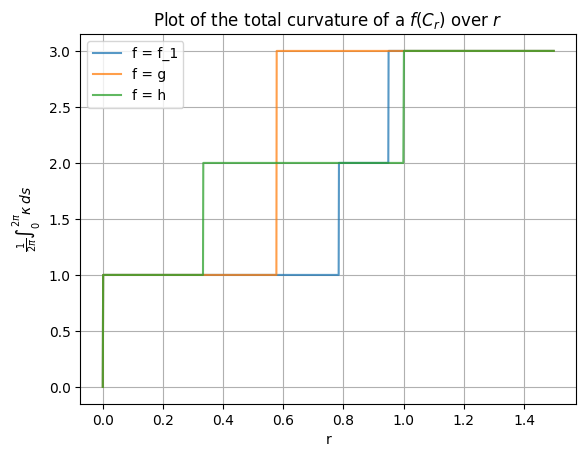
\includegraphics[width=1.0\linewidth]{images/winding_number.png}
    \caption{Dividing the total curvature by \(2\pi\) gives the turning number of a curve.}
\end{figure}

For a general polynomial, \(f(z)\) we have the following identity:
\[ \frac{1}{2\pi}\int_{f(C_r)} \kappa\,ds = N, \]
where \(N\) is the turning number of the curve which is equivalently the winding number of the unit tangent vector around the origin, or the degree of the map assigning each point of \(f(C_r)\) to a unit tangent vector. This fact is closely related to the argument principle: given a meromorphic function \(F\) on a contour \(\gamma\), if \(\gamma\) avoids all the zeros and poles of \(F\), then
\[ \frac{1}{2\pi i}\int_{\gamma} \frac{F'(z)}{F(z)}\,dz = Z - P, \]
where \(Z\) and \(P\) respectively count the number of zeros and poles of \(F\) enclosed inside the contour \(\gamma\). 

To see this, consider the map \(\mathbf{x}'(\varphi)\). As \(\varphi\) goes from \(0\) to \(2\pi\), \(z(\varphi)\) traces out the circle \(C_r\), hence \(\mathbf{x}'(\varphi)\) traces out a new closed curve \(D_r\) in the complex plane, representing the tangent vectors. The winding number with respect to the origin is defined as
\[ \frac{1}{2\pi i}\int_{D_r} \frac{d\zeta}{\zeta} = \frac{1}{2\pi i}[\log(\mathbf{x}''(2\pi)) - \log(\mathbf{x}''(0))], \]
where \(\zeta = \mathbf{x}'(\varphi)\) and \(\frac{d\log\zeta}{d\varphi} = \frac{1}{\zeta}\frac{d\zeta}{d\varphi}\). Since \(\log\zeta = \log|\zeta| + i\arg\zeta\), this integral now becomes
\[ \frac{1}{2\pi i}\int_{D_r} \frac{d\zeta}{\zeta} = \frac{1}{2\pi}[\arg(\mathbf{x}''(2\pi)) - \arg(\mathbf{x}''(0))] = \frac{1}{2\pi}\int_{f(C_r)} \kappa\,ds. \]
We set \(F(z) = \mathbf{x}'(z) = izf'(z)\) which, as a polynomial has no poles in the complex plane. The zeros occur precisely when \(z = 0\) or at a critical point of \(f\). The argument principle states that the winding number of \(F\) around the origin is equal to the number of zeros of \(f'\) inside \(C_r\) plus \(1\), assuming \(f'(z) \neq 0\).

\section{Outlook}

We have seen one specific result of differential geometry, namely that the total curvature of a curve is equal to its turning number. Using similar methods, we can see other properties of curves, such as the isoperimetric inequalities, or perhaps properties of surfaces such as Gauss-Bonnet or the Euler characteristic.


\end{document}
